% Fresnel paper for ISWC05

% based on LLNCS.DEM the demonstration file of
% the LaTeX macro package from Springer-Verlag
% for Lecture Notes in Computer Science,
% version 2.2 for LaTeX2e
%
\documentclass{llncs}
%
\usepackage{makeidx}  % allows for indexgeneration
\usepackage{graphicx}
%
\begin{document}
%
\newcommand{\rdf}[1]{{\small \texttt{#1}}}

\frontmatter          % for the preliminaries
%
\pagestyle{headings}  % switches on printing of running heads
\mainmatter              % start of the contributions
%
\title{Fresnel - A Browser-Independent Display Vocabulary for RDF}
%
\titlerunning{Fresnel - A browser-independent Display Vocabulary for RDF}
% abbreviated title (for running head)
%                                     also used for the TOC unless
%                                     \toctitle is used
%
\author{Christian Bizer\inst{1} \and Ryan Lee\inst{2} \and Stefano Mazzocchi\inst{3} \and Emmanuel Pietriga\inst{4}}
%
%\authorrunning{Bizer et al.}   % abbreviated author list (for running head)
%
%%%% modified list of authors for the TOC (add the affiliations)
\tocauthor{Chris Bizer (Berlin),
Ryan Lee (MIT),
Stefano Mazzocchi (MIT Libraries),
Emmanuel Pietriga (INRIA)}
%
\institute{Freie Universit\"at Berlin, Germany \\
\email{chris@bizer.de}
\and
W3C/MIT CSAIL, Cambridge, USA\\
\email{ryanlee@w3.org}
\and
MIT Libraries, Cambridge, USA\\
\email{stefanom@mit.edu}
\and
INRIA \& Laboratoire de Recherche en Informatique (LRI), Orsay, France\\
\email{emmanuel.pietriga@inria.fr}
}

\maketitle

%--------------------------------------------------------------------
\begin{abstract}
Todo: Change for new structure of paper: 1. There are different approaches, 2. Abstract Selection and Styling as common problems, 3. Developed Fresnel as a browser-independent ontology to handle these problems in order to faciliate the exchange of display knowledge.

Presenting Semantic Web content in a human-readable way consists in addressing two issues: specifying {\em what} information contained in an RDF graph should be presented and {\em how} this information should be presented. Each RDF browser or visualization tool currently relies on its own ad hoc mechanisms and vocabularies for addressing these issues, making it impossible to share RDF presentation knowledge across applications. Recognizing the general need for displaying RDF content and wanting to avoid reinventing the wheel with each new tool, we developed Fresnel as a browser-independent vocabulary of core RDF display concepts applicable across different representation paradigms. Fresnel's two foundational concepts are lenses and styles. Lenses define which properties of an RDF resource, or group of related resources, are displayed and how those properties are ordered. Styles determine how resources and properties are rendered by specifying styling attributes, making use of existing languages such as CSS and SVG wherever possible. In this paper describe the Fresnel display vocabulary and show how Fresnel is used within different RDF browsers, including Longwell and IsaViz.
\end{abstract}

%--------------------------------------------------------------------
%--------------------------------------------------------------------
\section{Introduction}

Software agents are the primary consumers of Semantic Web content. RDF is thus designed to facilitate machine interpretability of information and does not define a visual presentation model since human readability is not one of its stated goals. However, RDF applications are not only about the semantic processing of information. Information coming from the Semantic Web, either directly from RDF repositories or as a result of complex processes, often must be presented to users. Displaying RDF data in a user-friendly manner is a problem addressed by various types of applications using different representation paradigms. Tools like IsaViz \cite{isaviz} and Welkin \cite{Welkin} represent RDF models as node-link diagrams, explicitly showing their graph structure. Other tools use nested box layouts (Longwell \cite{simile}) or table-like layouts (Brownsauce \cite{Steer03}, Noadster \cite{Rutledge05}, Swoop \cite{MindSwap05}) for displaying properties of RDF resources with varying levels of details. A third approach combines these paradigms and extends them with specialized user interface widgets designed for specific information items like calendar data, tree structures, or even DNA sequences, providing advanced navigation tools and other interaction capabilities (Haystack \cite{Quan04}, mSpace\cite{mspace2005}).

Such applications are confronted with the same two issues, independently of the underlying representation paradigm and interface capabilities: selecting what content to show and specifying how to format and style this content. Each application takes its own approach and defines its own vocabulary to specify how to present data to users. As with other kinds of knowledge, we believe that being able to share what we consider {\em presentation knowledge} makes sense in the context of the Semantic Web and that being able to exchange and reuse presentation knowledge between browsers and other visualization applications will benefit both programmers and end users. However, the current diversity of approaches and vocabularies for representing this knowledge makes such exchange and reuse difficult at best, if not impossible.

\subsection{Current methods for specifying presentation knowledge}

Early RDF visualization tools rendered RDF models in a predefined, non-custo\-mizable way \cite{Steer03}. Recent tools provide more flexible visualizations that can be customized by writing style sheets, transformations, or templates, following either a declarative or a procedural approach.

Procedural approaches consider the presentation process as a series of transformation steps. One such approach consists of using XSLT to transform RDF graphs encoded as RDF/XML trees in an environment such as Cocoon \cite{cocoon05}. Authoring XSLT templates and XPath expressions to handle arbitrary RDF/XML is complex, if not impossible, considering the many potential serializations of a given RDF graph and the present lack of a commonly accepted RDF canonicalization in XML \cite{Carroll04}. This problem has been partly addressed by Xenon \cite{quan05}, an RDF style sheet ontology that builds on the ideas of XSLT but combines a recursive template mechanism with SPARQL as an RDF-specific selector language. Xenon succeeds in addressing XSLT's RDF canonicalization problem but still has a drawback common to all procedural approaches, that transformation rules are tied to a specific display paradigm and output format preventing the reuse of presentation knowledge across applications.

Declarative approaches are based on formatting and styling rules applied to a generic representation of the content. They can be compared to XHTML+CSS, which has been successful for the classic Web. The Haystack Slide ontology \cite{HaystackUI03}, used to describe how Haystack display widgets are laid out, is one example. Another is IsaViz's Graph Style Sheets \cite{gss03}, which modifies the formatting, styling, and visibility of RDF graph elements represented as node-link diagrams. The main drawback of the declarative approaches developed so far is that they make strong assumptions about, and are thus tied to, the specific display paradigm for which they have been developed and are therefore unlikely to be meaningful across different representation paradigms.

\subsection{Toward the specification of presentation knowledge}

Providing a single global view of all the information contained in an RDF model is often not useful. The amount of data makes it difficult to extract information relevant to the current task and represents a significant cognitive overload for the user. From an abstract perspective, the first step of the presentation process thus consists in restricting the visualization to small but cohesive parts of the RDF graph, similarly to views in the database world or RMM slices \cite{Isakowitz:1995:RMS}. Users can then select other points of interest by navigating in the model through hyperlinks and refine the selection with paradigms such as faceted browsing (e.g. Longwell \cite{simile}). But identifying what content to show is not sufficient for making a human-friendly presentation from the information. To achieve this goal, the selected content items must be laid out properly and rendered with graphical attributes that favor legibility in order to facilitate general understanding of the displayed information. Relying solely on the content's structure and exploiting knowledge contained in the schema associated with the data is insufficient for producing sophisticated visualizations. The second step thus consists in formatting and styling selected content items.

Fresnel's goal is to provide an RDF vocabulary to model information about how to present Semantic Web content to users (i.e., {\em what } content to show, and {\em how} to show it) as presentation knowledge that can be exchanged and reused between browsers and other visualization applications. However, we do not expect all applications, which do not necessarily rely on the same representation paradigms and formats, to exchange and reuse all formatting and styling instructions as they might not always be appropriate, depending on the underlying representation paradigm. We thus identified a set of core presentation concepts that are applicable across applications and which form the core modules of Fresnel. On top of these modules, we have also begun to define additional Fresnel vocabulary items which are grouped in extension modules. The remainder of this article mainly focuses on the core selection and formatting modules. More information about extension modules can be found in the Fresnel User Manual \cite{fresnel05}.



%--------------------------------------------------------------------
%--------------------------------------------------------------------
\section{Related Work}

Early RDF visualization tools rendered RDF models in a predefined, non-customizable way \cite{Steer03}. Recent tools provide more flexible visualizations, which can be customized by writing style sheets, transformations or templates for specific RDF vocabularies, following either a declarative or a procedural approach.

Procedural approaches encode presentation knowledge as a series of transformation steps. One approach from this category is using XSLT to transform RDF/XML-encoded RDF graphs in an environment such as Cocoon \cite{cocoon05}. Authoring XSLT templates and XPath expressions to handle arbitrary RDF/XML is complex, if not impossible, considering the many potential serializations of a given RDF graph and the present lack of a commonly accepted RDF canonicalization in XML \cite{Carroll04}. This problem is addressed by Xenon \cite{quan05}, an RDF stylesheet ontology that builds on the ideas of XSLT, but combines recursive templating mechanisms with SPARQL as an RDF-specific selector language. Xenon succeeds in addressing XSLT's RDF canonicalization problem but still has the drawback - as all procedural approaches - that transformation rules are very closely bound to a specific display paradigm or output format preventing the reuse of presentation knowledge across applications. 

Declarative approaches represent presentation knowledge as a set of generic selection and formatting instructions; trying to copy the ideas of HTML and CSS which where successful for the classic Web. One example from this category is the Haystack Slide ontology \cite{HaystackUI03}, which is used to describe how Haystack display widgets are laid out. A further example are IsaViz's node-and-arc oriented Graph Style Sheets\cite{gss03}. All declarative approaches are having in common that they encode presentation knowledge in a way which is closely bound to the display paradigm and presentation capabilities of the browser for which they have been developed and thus is not very meaningful for other browsers.

%--------------------------------------------------------------------
%--------------------------------------------------------------------
\section{Fresnel Lens Vocabulary}

Fresnel lenses describe which properties of RDF resources are shown and how these properties are ordered. For example, a summary lens for a class representing people such as \rdf{foaf:Person} might display the name and the email address properties of each person. 

The \rdf{fresnel:lensDomain} property specifies the set of instances to which a lens is applicable. A lens domain can be defined by one or more classes, in which case the lens is applicable to instances of these classes. A domain can also be defined by a set of instances using an FSL or SPARQL selector (see section \ref{selectors}). Such selectors are used to specify a lens domain in terms of the existence (or lack) of properties and values associated with the resources that constitute the domain. They thus make it possible to associate lenses with untyped RDF resources, which can and do occur in real-world models as \rdf{rdf:type} properties are not mandatory. 

In a distributed and open environment, browsers confronted with unknown RDF vocabularies for which no stylesheet is available locally can query repositories for appropriate lenses. Queries are made on the \rdf{fresnel:lensDomain} property of available lenses in order to evaluate their ability to handle the resources to be presented. Queries can also make use of the \rdf{fresnel:purpose} property, which encodes metadata about lenses, more specifically their intended use and characteristics. The purpose property can state that a lens is the default lens for a given class, or that it gives a good one-line summary (e.g. a label) of resources, etc. The following example shows a lens applicable to resources identifying persons, as defined by the Friend-of-a-Friend (FOAF) vocabulary \cite{foaf}.
% try to make sure this example stays on one page
\begin{small}
\begin{verbatim}
:PersonLens a fresnel:Lens ;
    fresnel:lensDomain foaf:Person ;
    fresnel:purpose fresnel:defaultLens ;
    fresnel:showProperties ( 
        foaf:name
        foaf:mbox
        [ a fresnel:PropertyDescription ;
          fresnel:property foaf:knows ;
          fresnel:depth "2"^^xsd:nonNegativeInteger ;
          fresnel:sublens :PersonLens ]
        fresnel:allProperties ) ;
    fresnel:hideProperties ( 
        rdfs:label 
        dc:title ) .
\end{verbatim}
\end{small}


\subsection{Property Selection and Ordering}

In the previous example\footnote{All examples in this paper use the Notation 3 syntax for RDF \cite{N3}.}, \rdf{fresnel:showProperties} and \rdf{fresnel:hideProperties} define which properties must be shown or hidden when the lens is used to display resources of type \rdf{foaf:Person}. The value of \rdf{showProperty} and \rdf{hideProperties} can either be a single URI reference identifying the property to show or hide, or a list of such URI references. Properties to show are displayed according to their order of appearance in the list that is the value of \rdf{fresnel:showProperties}.

Special value \rdf{fresnel:allProperties} can be used to avoid having to explicitly name each property that should be displayed. This value is also useful when the list of properties that can potentially be associated with resources handled by a lens is unknown to the lens' author but should nevertheless be displayed. When it appears as a member of the list of properties to be shown by a lens, \rdf{fresnel:allProperties} designates the set of properties that are not explicitly designated by other property URI references in the list, except for properties that appear in the list of properties to hide (\rdf{fresnel:hideProperties}). These unnamed properties are displayed according to the position of \rdf{fresnel:allProperties} in the list. In the previous example, \rdf{foaf:name}, \rdf{foaf:mbox} and \rdf{foaf:knows} properties are displayed in this order, before all other properties, which appear next as indicated by the presence of \rdf{fresnel:allProperties} at the end of the list of properties to be shown. Properties \rdf{rdfs:label} and \rdf{dc:title} will not be displayed even if they exist, as they are explicitly declared as hidden.

Fresnel provides two additional constructs for specifying what properties of resources to display. The first one handles the potential irregularity of RDF data coming from the fact that different authors might use similar terms coming from different vocabularies to make equivalent statements. Sets of such similar properties can be grouped in ordered lists and said to be \rdf{fresnel:alternateProperties}. For instance, \rdf{foaf:name}, \rdf{dc:title}, \rdf{rdfs:label} can be considered by a lens as giving the same information about resources. A browser using this lens will then try to display the resource's \rdf{foaf:name}. If the latter does not exist, the browser will look for \rdf{dc:title} and \rdf{rdfs:label} in this order. The second Fresnel construct, \rdf{fresnel:mergeProperties}, is used to merge the values of related properties (e.g. \rdf{foaf:homepage} and \rdf{foaf:workHomepage}) into one single set of values for presentation purposes.

\subsection{Lenses and Sublenses}

It is often desirable to display cohesive parts of RDF graphs involving a group of related resources, such as a person together with her projects and papers. Cohesive parts of graphs are defined by relating lenses using the \rdf{fresnel:sublens} property. In the previous example, a sublens is used to display persons that are known by the current person. The \rdf{fresnel:sublens} property states that lens \rdf{:PersonLens} should be used to display the value of \rdf{foaf:knows} properties. As this introduces recursiveness in the lens definition, property \rdf{fresnel:depth} is used to specify the closure value. In the end, this example lens will display persons together with her friends and the persons known by her friends.

As shown in this example, lens URIs are used to explicitly identify what lens to use as sublenses for presenting property values. Appropriate sublenses can also be identified by expressing constraints on lens definitions (domain, purpose, etc.) using a Fresnel Selector Expression or a SPARQL query evaluated against the set of lenses available to the browser.

%Naming the properties to show ultimately results in an output of statements with a lens-matched resource as the subject of each statement.  The objects of the output statements may also be resources; to describe how to display statement objects, a {\em sublens} may be used.


%--------------------------------------------------------------------
\section{Fresnel Style Vocabulary}
\label{fsStyle}

Fresnel lenses specify what information to display but do not give any indication about how to display it. The representation of selected information items mainly depends on the browser's representation paradigm (e.g. nested box layout, table layout, node-link diagrams, advanced widget-based UI, etc.) which defines a default rendering method. The final rendering can however be customized by associating specific styling and layout instructions to elements of the representation, as CSS styling rules do for elements of HTML documents.

Fresnel styling rules are made of a selector and a set of associated styling instructions. Following the lens approach, property \rdf{fresnel:styleDomain} takes a selector as its value (see section \ref{selectors}) and is used to declare the set of RDF properties or resources to which styling instructions apply. Styling instructions themselves are expressed using either Fresnel constructs for RDF-specific styling concepts, or existing languages (CSS \cite{CSS} and SVG \cite{SVG}) for fonts, colors, margins, and borders. 

\subsection{Fresnel Styling Instructions}

Fresnel styling instructions are expressed in RDF and can be used to specify RDF-specific styling concepts such as how properties are labeled and grouped. Fresnel's default behavior is to label properties using the declared \rdf{rdfs:label} of the property type. If this information is not available, then the property's URI is displayed instead. This behavior can be customized thanks to property \rdf{fresnel:label}, which defines whether a property label is displayed (\rdf{fresnel:show}) or not (\rdf{fresnel:none}, see figure \ref{styleCode}), or if it has a fixed custom literal value.

The presentation of property values can also be customized. Fresnel's default property value display method consists in searching for a lens matching the value's type and characterized by purpose \rdf{fresnel:labelLens}. Some kinds of values are however better represented by other means than labels, and it is therefore desirable to specify alternate behaviors. Instruction \rdf{fresnel:value} can be associated with different Fresnel behaviors, such as \rdf{fresnel:image} (see figure \ref{styleCode}) which states that the value to be represented is a URI reference identifying a bitmap image  whose content should be fetched over the Web in order to be displayed. Property values can be grouped, and additional content such as commas and an ending period can be specified using instructions \rdf{fresnel:contentAfter} and \rdf{fresnel:contentLast} to present multi-valued properties. Instruction \rdf{fresnel: contentNoValue} can be used to generate fixed content signaling missing values.

\subsection{CSS and SVG Styling Instructions}

As the set of display elements and layout method depend entirely on the browser's representation paradigm, Fresnel only defines an abstract representation model that can be interpreted and instantiated differently by every application. This abstract model is used to identify the elements of the output document to which CSS and SVG styling instructions can be hooked in a cross-application and cross-format manner. In the abstract model, the container box is the outermost Fresnel container. It identifies the region of the display that contains a group of principal resources to be presented. The container box contains resource and property boxes which identify regions of the display that are respectively associated with resources themselves and their properties. Property boxes are further decomposed as a label box and one or more value boxes which respectively hold the property's label and its value(s). Styling instructions can then be hooked to these presentation elements. The instructions are specified as literal values of properties \rdf{fresnel:containerStyle}, \rdf{resourceStyle}, \rdf{propertyStyle}, \rdf{labelStyle} and \rdf{valueStyle}. Such literal values can contain either styling instructions directly (see figure \ref{styleCode}), or a CSS class name referencing a rule in an external stylesheet.

\begin{figure}
    \begin{center}
      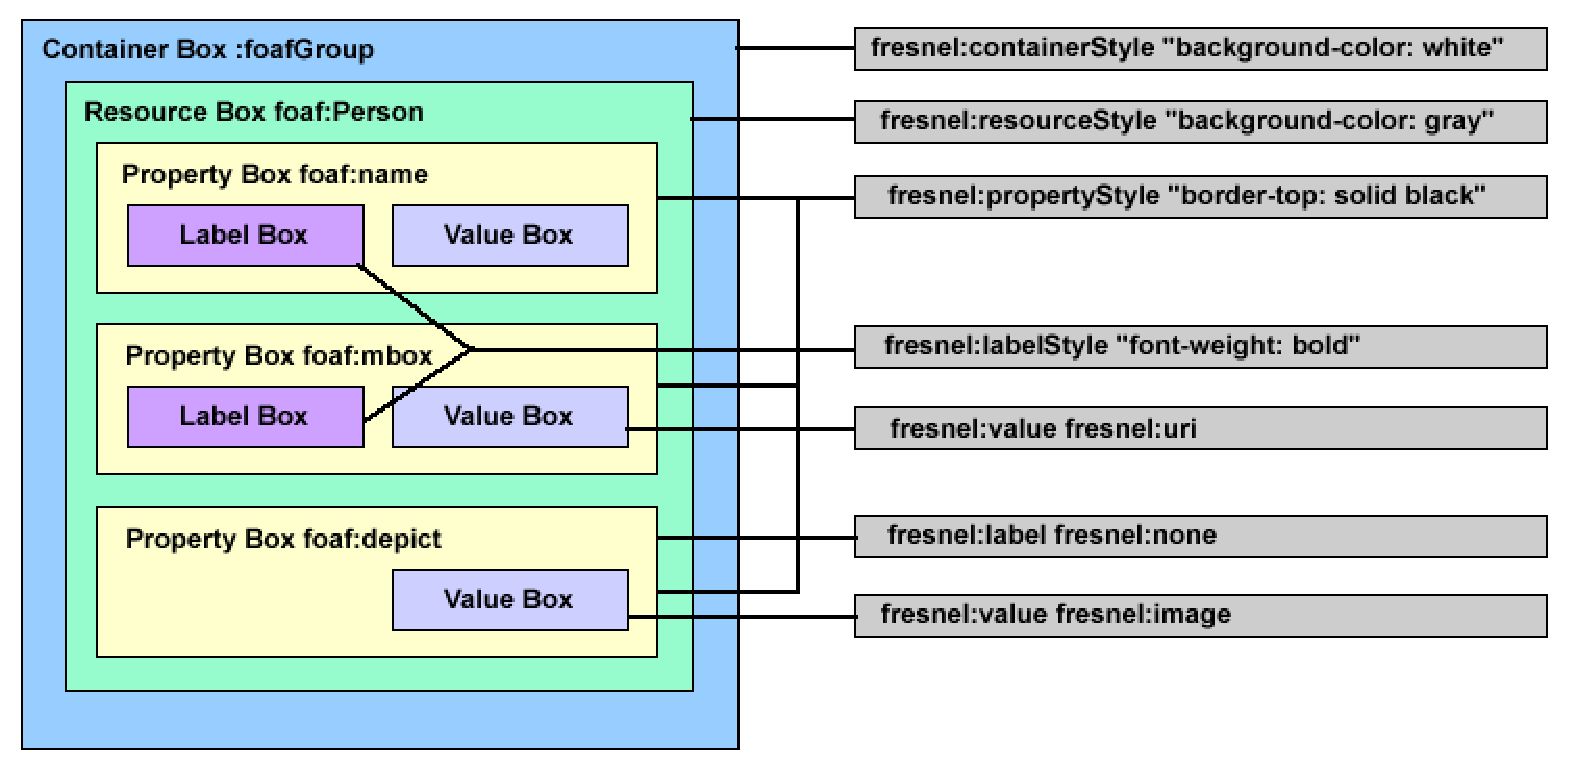
\includegraphics[width=10cm]{boxmodelexample.pdf}
    \end{center}
    \vspace{-0.3cm}
    \caption{Box model with attached styling instructions}
    \label{boxModel}
\end{figure}

Figure \ref{boxModel} contains a schematic view of how the abstract Fresnel model could be interpreted and instantiated by a Web-based browser using the nested box representation paradigm. 

\begin{figure}
    \begin{tabular}{c|c}
      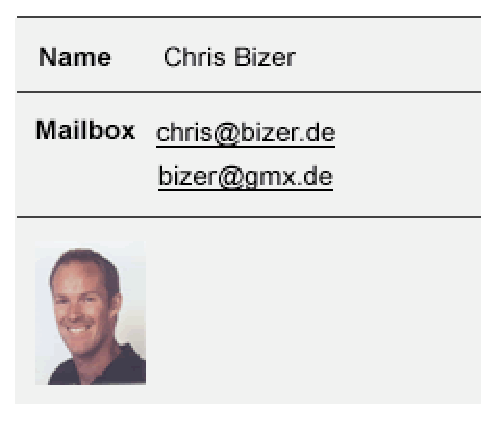
\includegraphics[height=4.3cm]{boxmodelexampleoutput.pdf} &
      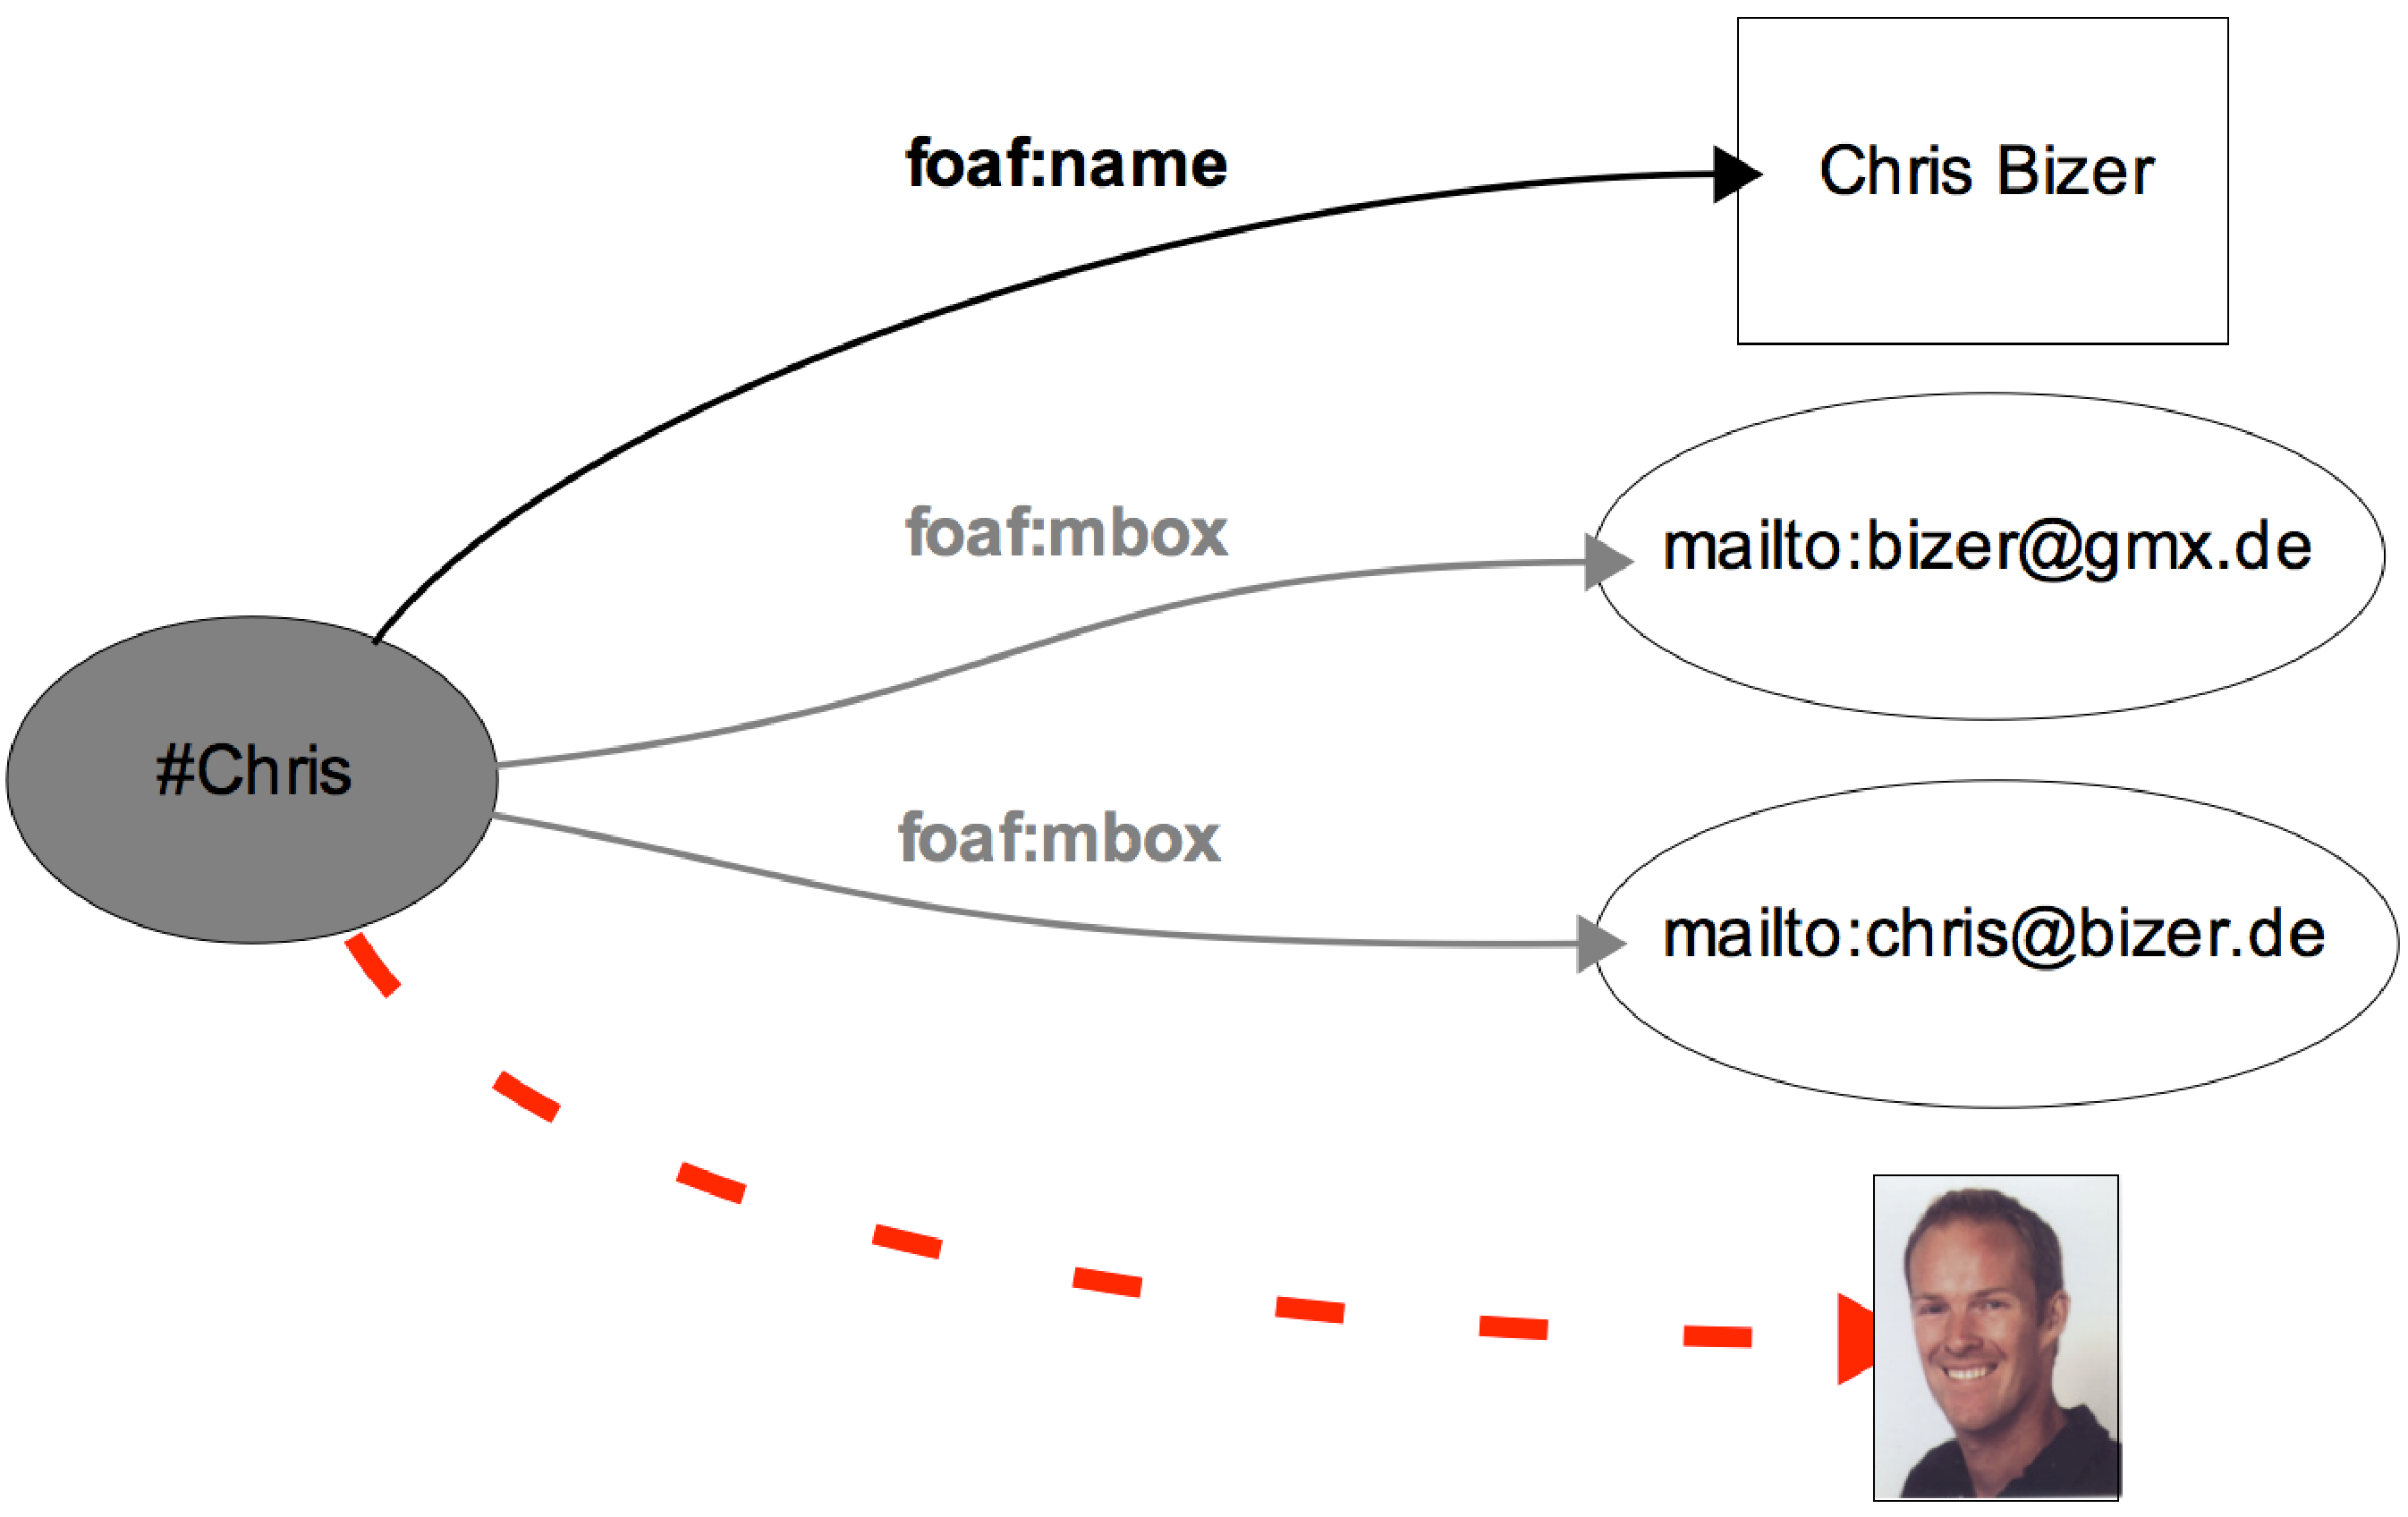
\includegraphics[height=4.3cm]{isv_scs.pdf} \\
      (a) & (b)\\
    \end{tabular}
    \caption{Two interpretations for two representation paradigms}
    \label{boxEx}
\end{figure}

Figure \ref{boxEx}-a shows a possible final rendering based on this model as it might be generated by Longwell. Note that the example model of figure \ref{boxModel} is just one possible instantiation of the abstract Fresnel model. The abstract presentation elements introduced above could be mapped to (possibly non-rectangular) shapes laid out in very different manners, depending on the browser's capabilities and fundamental representation paradigm.

Figure \ref{boxEx}-b shows a different final rendering produced by IsaViz\footnote{This Fresnel presentation was simulated with a GSS stylesheet \cite{Pietriga03} as IsaViz does not support all Fresnel features at the time of submission.}, based on another instantiation of the Fresnel abstract representation model relying on node-link diagrams. The two examples of figure \ref{boxEx} thus illustrate two presentations, by two browsers based on different representation paradigms, of the same data using the same Fresnel lens and styling instructions. But other representation models based on  other paradigms are possible. For instance, a server producing HTML pages for user agents that do not support CSS might choose a basic table-based representation of RDF triples and interpret the property and value boxes as cells of a table row.


The style example of figure \ref{styleCode} specifies that \rdf{foaf:depiction} property values should be displayed as images with a black border, but no property label. Additional styling instructions are used to further customize \rdf{foaf:depiction} properties' appearance. Some of these instructions might be ignored by browsers depending on their relevance with respect to the underlying representation para\-digm. For instance, the border-top instruction will be interpreted by browsers based on a standard box model, whereas it is likely to be ignored by visualization tools such as IsaViz which is more likely to interpret stroke-related instructions.

\vspace{-0.5cm}

\begin{figure}
\begin{small}
\begin{verbatim}
:depictStyle rdf:type fresnel:Style ;
    fresnel:styleDomain foaf:depiction ;
    fresnel:label fresnel:none ;
    fresnel:value fresnel:image ;
    fresnel:propertyStyle "border-top: solid 
                           black"^^fresnel:StylingInstructions;
    fresnel:labelStyle "stroke-dasharray: 10px,20px; stroke-width: 2px; 
                        stroke: red"^^fresnel:StylingInstructions ;
    fresnel:valueStyle "border: solid black"^^fresnel:StylingInstructions.
\end{verbatim}
\end{small}
\vspace{-0.3cm}
\caption{Fresnel style for property \rdf{foaf:depiction}}
\label{styleCode}
\end{figure}



%--------------------------------------------------------------------
\section{Fresnel Selectors}
\label{selectors}

Selection in Fresnel occurs when specifying the domain of a lens or format and when specifying what properties of a resource a lens should show. Such selection expressions identify elements of the RDF model to be presented; in other words, specific nodes and arcs in the graph. As we expect selection conditions to be of varying complexity, we allow them to be expressed using different languages in an attempt to balance expressive power against ease of use.

\subsection{Basic Selectors}

The simplest selectors, called basic selectors, take the form of plain URI references as shown in section \ref{fresnelov}. Depending on whether they are used as values of \rdf{fresnel:instan\-ceLensDomain} or \rdf{fresnel:classLensDomain}, these URI references are interpreted respectively either as:
\begin{itemize}
\item URI equality constraints (the resource to be selected should be identified by this URI),
\item or type constraints (the resources to be selected should be instances of the class identified by this URI).
\end{itemize}

Basic selectors are also used to identify properties, which are used for instance as values of \rdf{fresnel:showProperties} or \rdf{fresnel:alternateProperties}.

%In the following example, property \rdf{fresnel:lensDomain} indicates that this lens should be used to display instances of class \rdf{foaf:Person}, i.e., resources that have an rdf:type property pointing at class (or at a subclass of \footnote{Subclass and subproperty relationships must be taken into account by the selection mechanism, provided that an RDF Schema or OWL ontology is available at runtime 
%for the associated vocabulary.}) \rdf{foaf:Person}. Property \rdf{fresnel:showProperties} takes as its value a list of URIs referencing RDF property types. Properties \rdf{foaf:name} and \rdf{foaf:depiction} of resources displayed by this lens should be shown. 

%\begin{small}
%\begin{verbatim}
%:PersonLens a fresnel:Lens ; 
%    fresnel:lensDomain foaf:Person ; 
%    fresnel:showProperties (
%        foaf:name 
%        foaf:depiction
%    ).
%\end{verbatim}
%\end{small}

Basic selectors are easy to use but have very limited expressive power. For instance, they cannot be used to specify that a lens should apply to all instances of class \rdf{foaf:Person} that are the subject of at least five \rdf{foaf:knows} statements. More powerful languages are required to express such selection constraints.

\subsection{Languages for Complex Selection Expressions}

Fresnel presentation designers can use two different languages for expressing complex selection expressions. The first option is the SPARQL query language for RDF \cite{sparql05}. In the context of Fresnel, SPARQL queries must always return exactly one result set, meaning that only one variable is allowed in the query's SELECT clause. Figure \ref{fslsparqlExample}-a gives an example of a lens whose domain is defined by a SPARQL expression. Alternatively, designers who prefer a more XPath-like approach, which proved to be a well-adapted selector language for XSLT, can use the Fresnel Selector Language (FSL). FSL is a language for modeling traversal paths in RDF graphs, designed to address the specific requirements of a selector language for Fresnel. It does not pretend to be a full so-called RDFPath language (contrary to XPR \cite{xpr06}, an extension of FSL) but tries to be as simple as possible, both from usability and implementation perspectives. FSL is strongly inspired by XPath \cite{xpath}, reusing many of its concepts and syntactic constructs while adapting them to RDF's graph-based data model. RDF models are considered directed labeled graphs according to RDF Concepts and Abstract Syntax \cite{rdfcas04}. FSL is therefore fully independent from any serialization. A lens definition using two FSL expressions is shown in Figure \ref{fslsparqlExample}-b. More information about FSL, including its grammar, data model and semantics is available in the FSL specification \cite{fsl05}.

\begin{figure}
%\begin{center}
\begin{scriptsize}
\begin{verbatim}
# (a) Lens for John Doe's mailboxes    (SPARQL)
:PersonLens a fresnel:Lens ;
            fresnel:instanceLensDomain
              "SELECT ?mbox WHERE ( ?x foaf:name 'John Doe' )
                                  ( ?x foaf:mbox ?mbox )"^^fresnel:sparqlSelector .

# (b) Lens for foaf:Person instances that know at least five other resources  (FSL)
:PersonLens a fresnel:Lens ;
            fresnel:instanceLensDomain
                       "foaf:Person[count(foaf:knows) >= 5]"^^fresnel:fslSelector ;
# and which shows the foaf:name property of all foaf:Person
# instances known by the current resource.
            fresnel:showProperties (
                         "foaf:knows/foaf:Person/foaf:name"^^fresnel:fslSelector) .
\end{verbatim}
\end{scriptsize}
%\end{center}
\vspace{-1em}
\caption{Examples of SPARQL and FSL expressions used in Fresnel lens definitions}
\label{fslsparqlExample}
\vspace{-1em}
\end{figure}


Applications implementing Fresnel are required to support basic selectors, and we expect a reasonable share of them to support the two other languages: SPARQL is gaining momentum as a W3C recommendation, and four open-source Java implementations of FSL are already available\footnote{http://dev.w3.org/cvsweb/java/classes/org/w3c/IsaViz/fresnel/} for HP's Jena Semantic Web Toolkit\footnote{http://jena.sourceforge.net}, for IsaViz (providing a visual FSL debugger) and for different versions of the Sesame RDF database\footnote{http://openrdf.org}.


%--------------------------------------------------------------------
\section{Fresnel Implementations}
\label{impl}

{\em Note to the reviewers: Fresnel is currently being implemented by several RDF visualization tools and there are further groups that are currently evaluating it and might descide to support Fresnel within their tools. This section reflects the current status of Fresnel implementations. We expect to update this section in the camera-ready version of this paper.}

Fresnel represents RDF display knowledge in an abstract and declarative manner. It provides high-level indications about how the data should be presented, but does not impose any constraint on the output format or any particular method or representation paradigm. It is therefore up to the browsers and applications to interpret Fresnel display knowledge according to their own representation paradigm. This section gives an overview of the Fresnel implementation efforts currently being conducted by several research groups.


%--------------------------------------------------------------------
%--------------------------------------------------------------------
% $Id: fresnelInLongwell.tex 1370 2005-04-20 20:34:09Z ryanlee $
\subsection{Longwell}

Longwell is a suite of RDF browsing applications written in Java and developed by the SIMILE project \cite{simile}.  Initial releases of Longwell implemented an {\em ad hoc} display vocabulary, amended as application needs arose.  The next major stable release, currently under development, will instead support the core selection terms from Fresnel.  Graph results from searches will be filtered through Fresnel lens definitions before being passed on to the rendering engine.  Also, a basic, experimental RDF browser, @@@unnamed, based off the same set of selection and browsing code, will implement all of the core Fresnel terms.

(@@@assuming a screenshot of longwell2 shows off the same data used in the IsaViz screenshot) As seen in the screenshot of Longwell \ref{longwellScreen}, the display of a \rdf{foaf:Person} using the (@@@which lens?) renders only what is specified in the lens in the order of specification; there is more data in the underlying collection involving contact information that is not shown.

Longwell generates XHTML and uses CSS to style data according to the CSS box model; this portion does not use Fresnel styling.


%--------------------------------------------------------------------
%--------------------------------------------------------------------
\subsection{IsaViz}

IsaViz \cite{isaviz} already implements a rendering engine that can interpret GSS style\-sheets \cite{Pietriga03} for styling RDF models represented as node-link diagrams. The new version (currently under development) features two presentation paradigms that both support Fresnel stylesheets: the default paradigm based on node-link diagrams, and a new paradigm based on the box model described in section \ref{fsStyle} which will take advantage of the zoomable user interface and semantic zooming capabilities associated with the graphical toolkit upon which the user interface is built \cite{Pietriga05a}.

@@@ Outline of interpretation in the node-link diagram representation

@@@ Mention alternate interpretation in the Semantic ZUI representation


%--------------------------------------------------------------------
%--------------------------------------------------------------------
\subsection{Other Implementations}

Another effort to implement Fresnel is the Arago RDF-browser. Arago is currently being developed at DERI and renders XHTML representations of RDF data\cite{Gassert05}. Another groups that are currently in the process of evaluating Fresnel and migh support it in their tools are the Haystack team at MIT\cite{Quan04} and the Noadster team at CWI\cite{Rutledge05}.




%--------------------------------------------------------------------
%--------------------------------------------------------------------
\section{Conclusion}

We have given an overview of Fresnel, a browser-independent, extensible vocabulary for modeling Semantic Web content presentation knowledge. Fresnel has been designed as a modularized, declarative language manipulating selection, formatting, and styling concepts that are applicable across representation paradigms, layout methods, and output formats. Fresnel core modules can be used to model presentation knowledge that is compatible and reusable between browsers and other types of Semantic Web information visualization~tools.

%I've added a ~ between the last two words to prevent tools from going on the next line.

Although core modules have been frozen for the time being, the Fresnel vocabulary remains a work in progress as new extension modules meeting special needs are being developed (e.g., for describing the {\em purpose} of lenses or adding new formatting capabilities). Extension modules are not necessarily aimed at being application- and paradigm-independent, as they might not be relevant in all cases; but their inclusion in Fresnel provides users with a unified framework for modeling presentation knowledge. 

Core modules are currently being implemented in various types of applications: SIMILE's Longwell \cite{simile} faceted browser, IsaViz \cite{isaviz} which represents RDF graphs as node-link diagrams, and Horus \cite{horus}, a PHP-based RDF browser. More information about Fresnel can be found on its web site\footnote{http://www.w3.org/2005/04/fresnel-info/}. Its development is an open, community-based effort and new contributors are welcome to participate in it.




%
% ---- Bibliography ----
%

\bibliographystyle{splncs}
\bibliography{fresnel}

\end{document}
